% ----------------------------------------------------------------------
%  Před psaním se důkladně seznamte s Pravidly pro vypracování protokolu!
% ----------------------------------------------------------------------

% ----------------------------------------------------------------------
%  Pracovní úkoly - opište přímo ze zadání
% ----------------------------------------------------------------------
\section{Pracovní úkoly}

\begin{enumerate}
\item Nastavte zesílení proporcionálního členu na 1 ($R_P=R'_P=10 \unit{k\Omega}$). Dále vyřaďte integrační ($R_I=\infty$ a $C_I=0 \unit{nF}$) a derivační člen ($C_D=\infty$ a $R_D=0 \unit{\Omega}$).
\item Změřte statickou charakteristiku soustavy v otevřené smyčce. Hodnoty vyneste do grafu (závislost otáček za minutu na řídící veličině). Rozsah řídící veličiny bude od -1.6 V do 1.6 V.
\begin{enumerate}
	\item Je tato charakteristika lineární nebo nelineární, případně v jakém rozsahu je lineární?
	\item Vyjádřete funkční závislost statické charakteristiky lineární funkcí.
\end{enumerate}
\item Změřte přechodovou charakteristiku soustavy v otevřené smyčce. Hodnoty vyneste do grafu (závislost napětí z tachogenerátoru na čase). Řídící veličina se skokově změní z 0.6 V na 1.6 V.
\item Dle změřené přechodové charakteristiky identifikujte strukturu a řád modelu soustavy.
\begin{enumerate}
	\item Jaká je obecná přenosová funkce tohoto modelu?
	\item Popište parametry modelu.
	\item Metodou experimentální identifikace odhadněte parametry modelu.
	\item Ověřte průběh přechodové charakteristiky modelu s naměřenými daty.
\end{enumerate}
\item Změřte amplitudovou a fázovou frekvenční charakteristiku soustavy v otevřené smyčce. Hodnoty vyneste do grafu (závislost amplitudy [dB] / fáze [stupně] na frekvenci [log f]). Frekvenční rozsah bude od 0.1 Hz do 5 Hz.
\begin{enumerate}
	\item Jaká je frekvence zlomu?
	\item Jaká je šířka pásma soustavy?
\end{enumerate}
\item Změřte přechodovou charakteristiku soustavy v uzavřené smyčce pouze s P regulátorem se zesílením 1. Hodnoty vyneste do grafu (závislost napětí z tachogenerátoru na čase). Porovnejte přechodové charakteristiky a časové konstanty se soustavou v otevřené smyčce. Jaká je trvalá regulační odchylka?
\item Změřte amplitudovou frekvenční charakteristiku soustavy v uzavřené smyčce. Hodnoty vyneste do grafu (závislost amplitudy [dB] na frekvenci [log f]). Frekvenční rozsah bude od 0.1 Hz do 5 Hz. Jaká je frekvence zlomu? Porovnejte amplitudovou frekvenční charakteristiku se soustavou v otevřené smyčce.
\item Metodou pokus-omyl zjistěte parametry regulátoru, aby trvalá regulační odchylka byla menší než 0.3 V (cca. 300 ot./min) a časová konstanta soustavy byla menší než 20 ms.
\end{enumerate}

% ----------------------------------------------------------------------
%  Použité pomůcky
% ----------------------------------------------------------------------

\newpage
\section{Sestavení experimentu}

Na obrázku Obr.\ref{fig:schema_reg} je vyobrazeno schéma regulované soustavy, na obrázku Obr.\ref{fig:schema_PID} pak schéma PID regulátoru.

\begin{figure}[H]
  \centering
  \subfloat[Schéma regulované soustavy.]{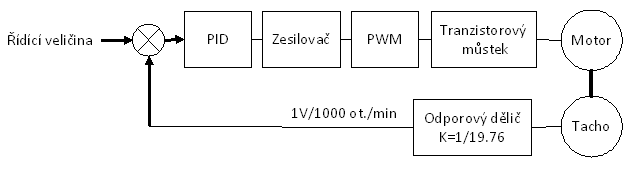
\includegraphics[width=0.5\textwidth]{img/schema_regulovane_soustavy.png}\label{fig:schema_reg}}
  \hfill
  \subfloat[Schéma PID regulátoru.]{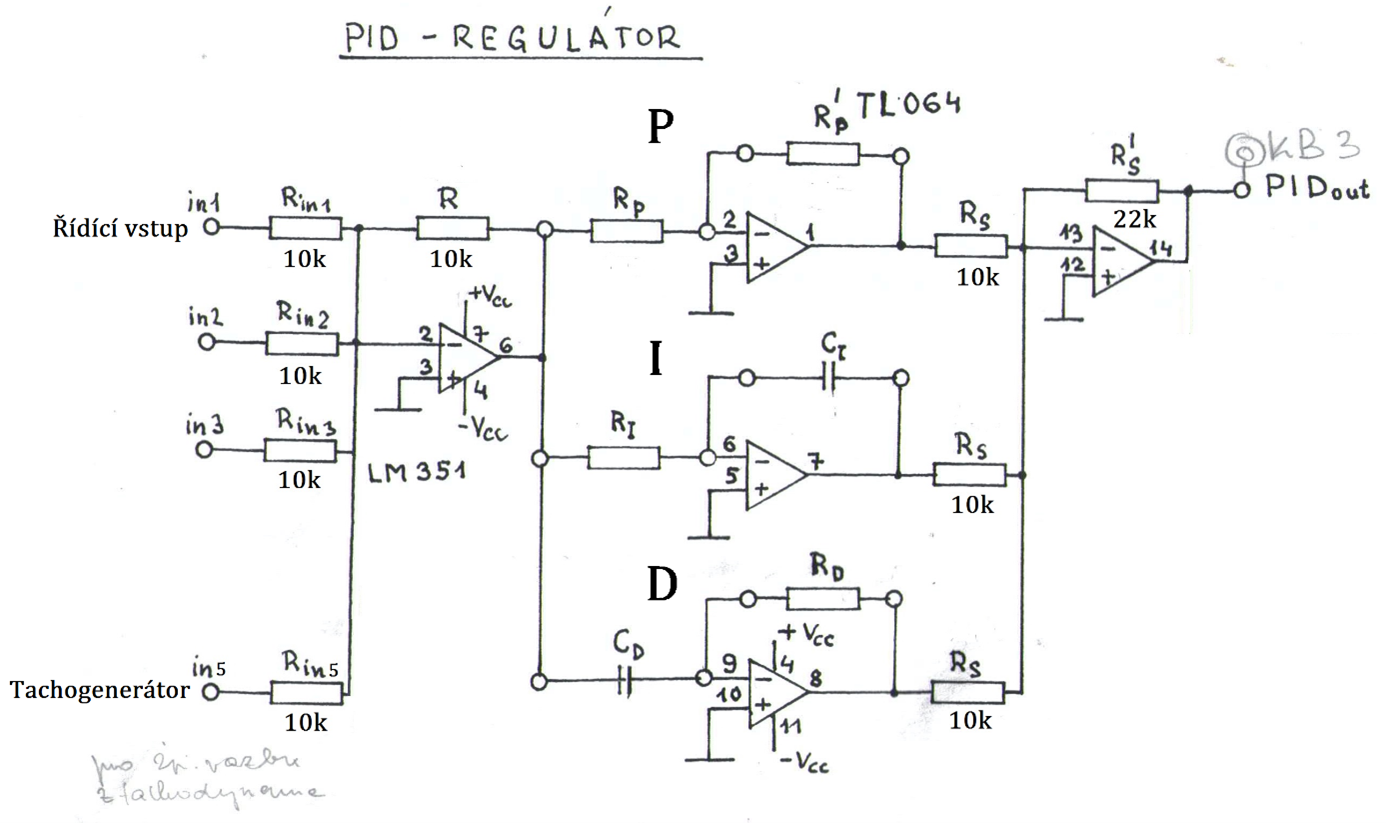
\includegraphics[width=0.5\textwidth]{img/schema_PID_regulatoru.png}\label{fig:schema_PID}}
  \caption{Sestavení experimentu.}
\end{figure}

%\begin{figure}[H]
%	\centering
%	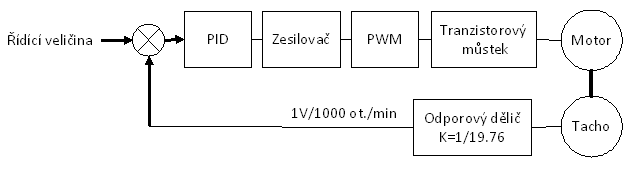
\includegraphics[scale = 0.5]{img/schema_regulovane_soustavy.png} 
%	\caption{Schéma regulované soustavy.} 
%	\label{fig:schema_reg}
%\end{figure}	

%\begin{figure}[H] 
%	\centering
%	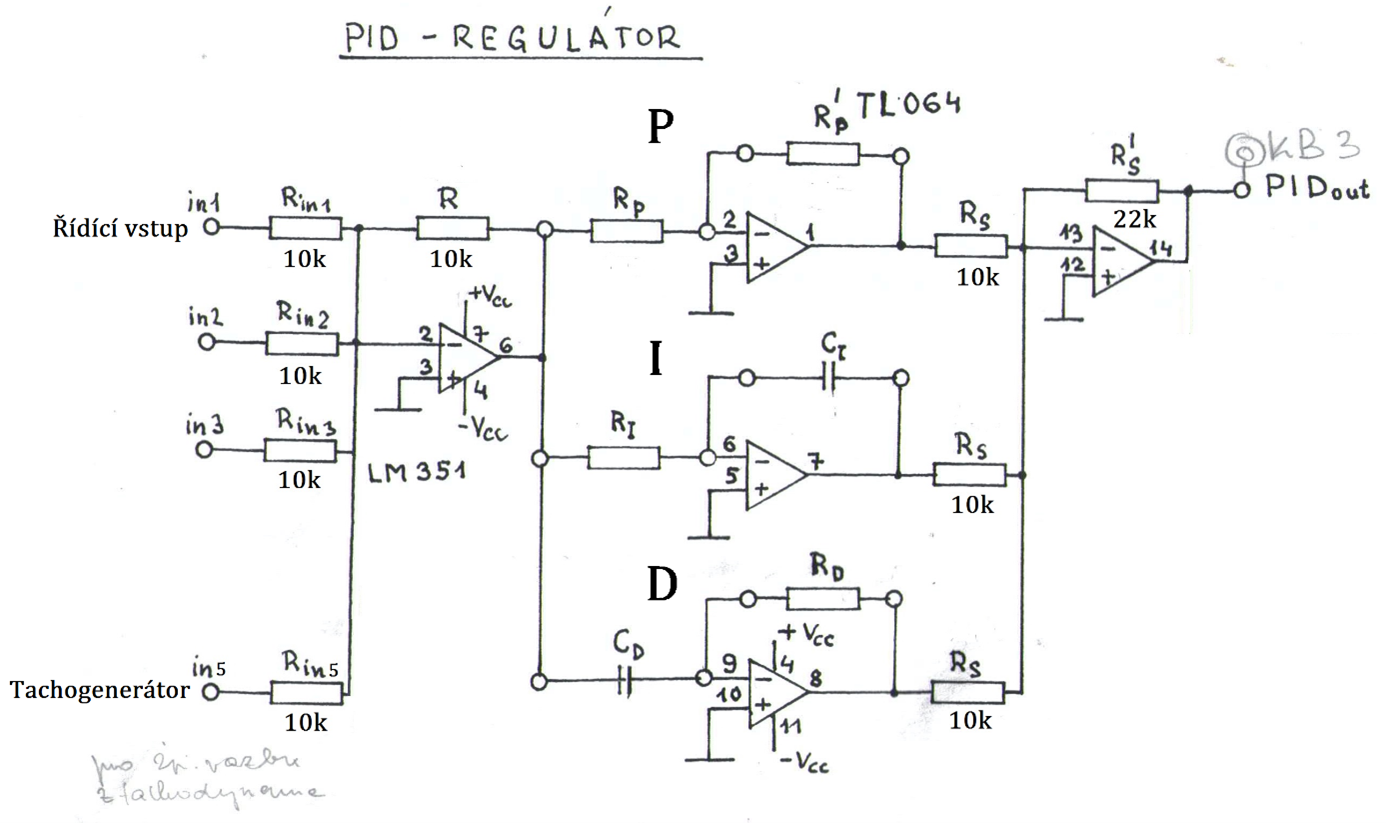
\includegraphics[scale = 0.7]{img/schema_PID_regulatoru.png} 
%	\caption{Schéma PID regulátoru.} 
%	\label{fig:schema_PID}
%\end{figure}		
		

% ----------------------------------------------------------------------
%  Teoretický úvod - vlastními slovy stručne popište fyzikální podstatu měření a uveďte základní vztahy použité ve vypracování
% ----------------------------------------------------------------------
%\section{Teoretický úvod}	

% ----------------------------------------------------------------------
%  Postup měření - vlastními slovy popište postup měření tak, aby bylo vaše měření reprodukovatelné 
% ----------------------------------------------------------------------
%\section{Postup měření}
			
% ----------------------------------------------------------------------
%  Naměřené hodnoty a samotné vypracování úkolu
% ----------------------------------------------------------------------	
			
\section{Vypracování}
	\subsection{Statická charakteristika v otevřené smyčce}
		V grafu na Obr.~\ref{fig:staticka} jsou vyneseny naměřené hodnoty statické charakteristiky soustavy v otevřené smyčce. 
		V celém rozsahu (-1.6 V - 1.6 V) statická charakteristika lineární není, avšak mezi -0.8V až -0.6V a poté 0.6V až 0.8 V ji za lineární považovat lze.
		Pro kladnou větev je funkční závislost statické charakteristiky dána předpisem $$y=(-11.9\pm 0.9)x+(-6.6\pm 0.7)$$ a pro zápornou větev pak $$y=(-10.9\pm 0.9)x+(6\pm 0.6),$$ 
		kde $y$ je výstupní veličina v mV a $x$ je vstupní veličina ve V. 
		\begin{figure}[H] 
			\centering
			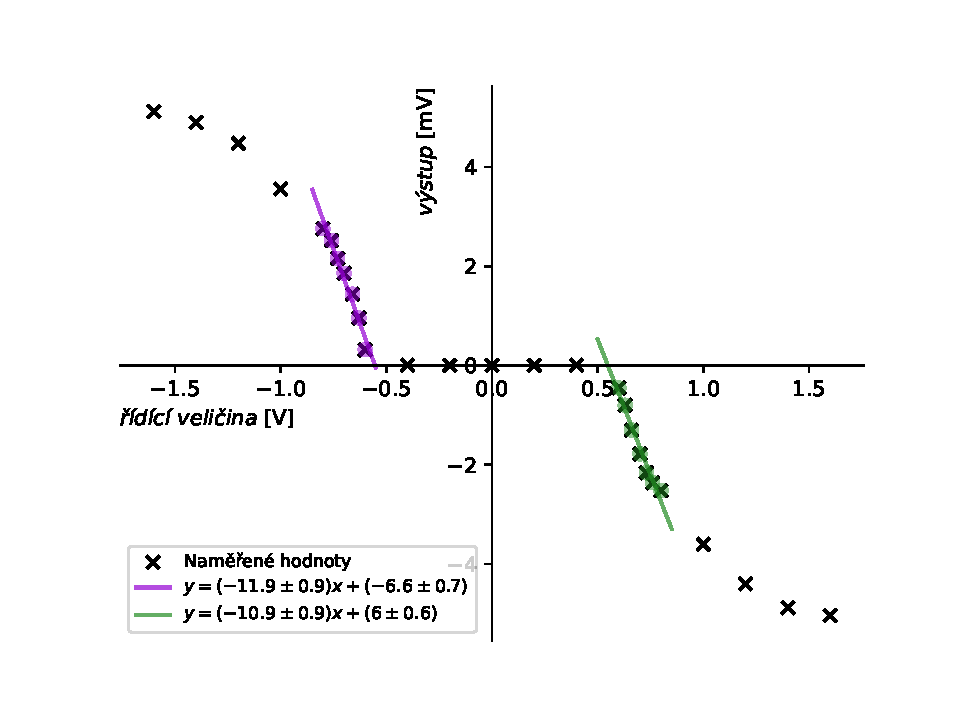
\includegraphics[width=0.6\textwidth]{img/graf_staticka.pdf} 
			\caption{Statická charakteristika soustavy v otevřené smyčce pro rozsah vstupní veličiny -1.6 V až 1.6 V. 
			Lineární část kladné větve (fialově) je proložena lineárním fitem $y=(-11.9\pm 0.9)x+(-6.6\pm 0.7)$, 
			lineární část záporné větve (zeleně) je fitována lineární funkcí $y=(-10.9\pm 0.9)x+(6\pm 0.6)$.} 
			\label{fig:staticka}
		\end{figure}


	\subsection{Přechodová charakteristika v otevřené smyčce}
		V grafu na Obr.~\ref{fig:prechodova} je vyobrazena přechodová charakteristika soustavy v otevřené smyčce (závislost napětí z tachogenerátoru na čase) 
		pro skokovou změnu řídící veličiny z 0.6 V na 1.6 V. Fialové body jsou hodnoty přechodové charakteristiky modelu získaného odhadem parametrů a zelené body jsou naměřená data.
		Dle tvaru přechodové charakteristiky lze usoudit, že se jedná o proporcionální systém 1. řádu, který je obecně popsán přenosovou funkcí
		\begin{equation}
			\frac{k}{T\cdot s + 1},
		\end{equation}
		kde $k$ je zesílení a $T$ je časová konstanta. Tyto parametry pro měřenou soustavu jsou přibližně $k=5$ a $T=150\unit{ms}$

		\begin{SCfigure}[1][h!]
			\centering
			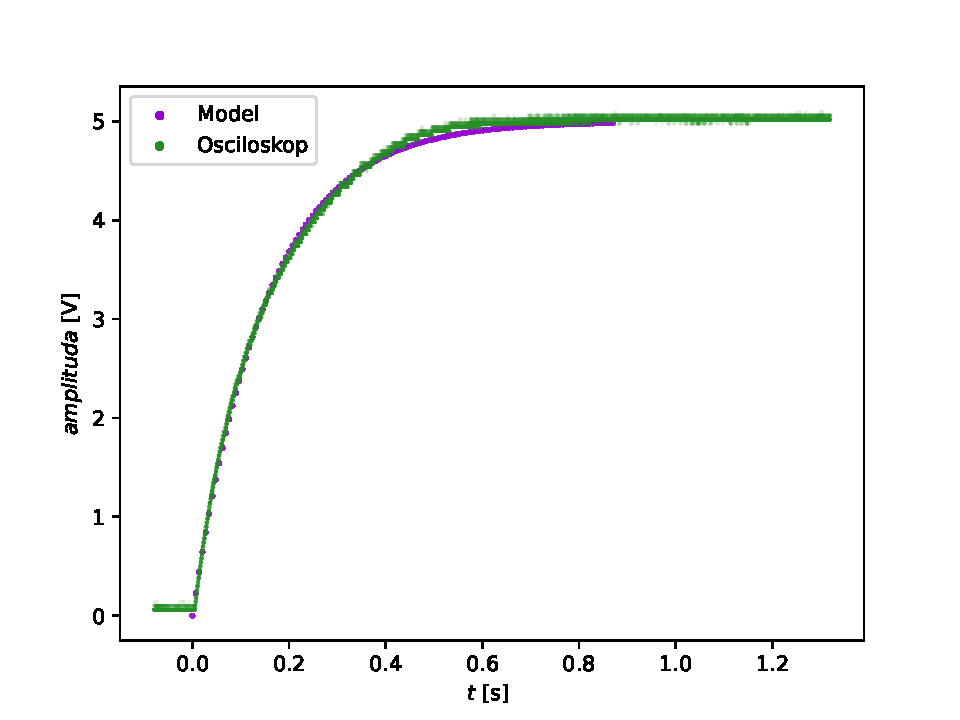
\includegraphics[width = 0.4\textwidth]{img/graf_prechodova.pdf} 
			\caption{Přechodová charakteristika soustavy v otevřené smyčce (závislost napětí z tachogenerátoru na čase) 
			pro skokovou změnu řídící veličiny z 0.6 V na 1.6 V. 
			Fialové body jsou hodnoty přechodové charakteristiky modelu získaného odhadem parametrů a zelené body jsou naměřená data.} 
			\label{fig:prechodova} 
		\end{SCfigure}

	\subsection{Amplitudová a fázová frekvenční charakteristika v otevřené smyčce}
		Graf frekvenční charakteristiky v otevřené smyčce je na Obr.~\ref{fig:bode_otevrena}. Horní graf představuje závislost amplitudy $A$ v dB na frekvenci $f$ (osa frekvence je logaritmická). Pro frekvence do přibližně 0.5 Hz je závislost víceméně konstantní, poté nastává zlom a průběh se mění na klesající funkci $A=(-20.5\pm 0.6)\log(f)+(-8\pm 0.2)$. Pokles o 3 dB nastává zhruba při frekvenci 0.6 Hz. Data byla vycentrována tak, aby konstantní část průběhu byla přibližně na hodnotě 0 dB. \\
		Spodní graf představuje závislost fázového posunu $\varphi$ na frekvenci $f$. Při přibližně 0.4 Hz je fázový posun roven 45$\deg$.

		\begin{figure}[H] 
			\centering
			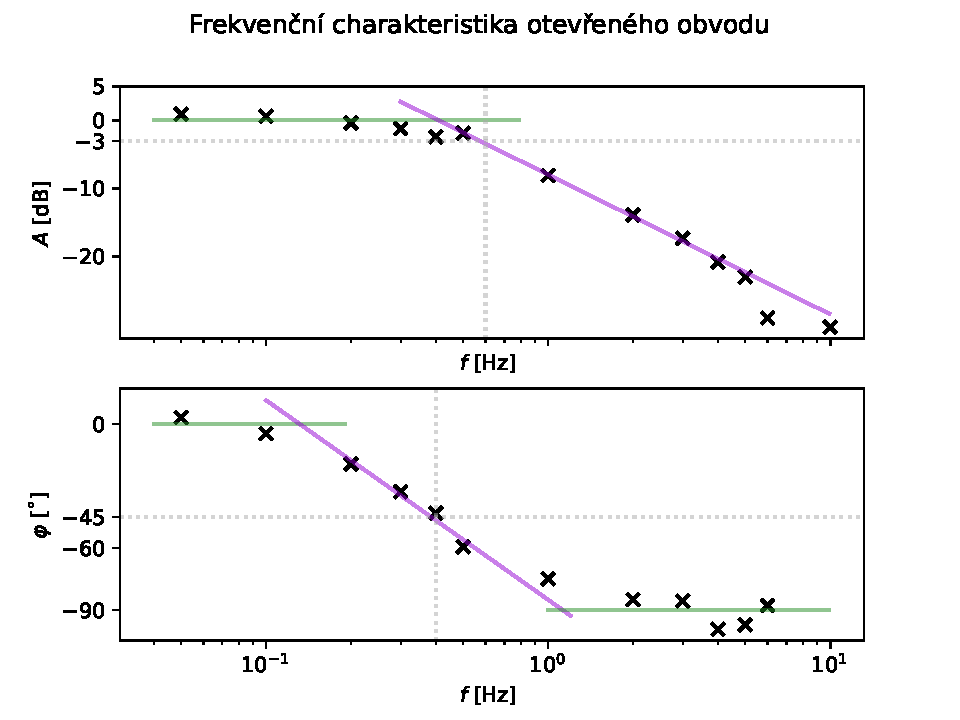
\includegraphics[scale=0.6]{img/graf_bode_otevrena.pdf} 
			\caption{Graf frekvenční charakteristiky v otevřené smyčce. Horní graf představuje závislost amplitudy $A$ v dB na frekvenci $f$ (osa frekvence je logaritmická). Pro frekvence do přibližně 1 Hz je závislost víceméně konstantní, poté nastává zlom a průběh se mění na klesající funkci $A=(-20.5\pm 0.6)\log(f)+(-8\pm 0.2)$. Data byla vycentrována tak, aby konstantní část průběhu byla přibližně na hodnotě 0 dB. Spodní graf představuje závislost fázového posunu $\varphi$ na frekvenci $f$.} 
			\label{fig:bode_otevrena}
		\end{figure}


	\subsection{Přechodová charakteristika v uzavřené smyčce}
		Na Obr.~\ref{fig:prechodova_uzavrena_k1} je snímek z osciloskopu zobrazující přechodovou charakteristiku v uzavřené smyčce. Měření bylo provedeno s nastavením zesílení P regulátoru na $k=1$, časová konstanta při tomto zesílení byla $T=34\unit{ms}$ a regulační odchylka byla 0.1 V.

		\begin{figure}[H] 
			\centering
			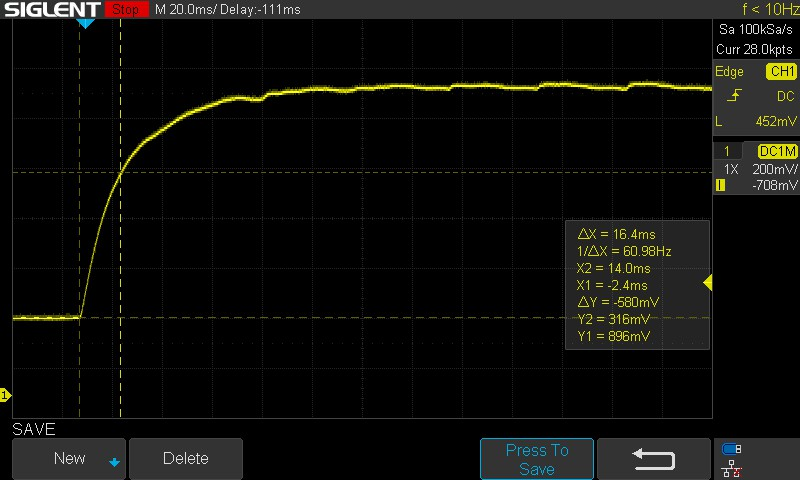
\includegraphics[width = 0.7\textwidth]{img/SDS00002.jpg} 
			\caption{Snímek z osciloskopu zobrazující přechodovou charakteristiku v uzavřené smyčce. Měření bylo provedeno s nastavením zesílení P regulátoru na $k=1$, časová konstanta při tomto zesílení byla $T=34\unit{ms}$ a regulační odchylka byla 0.1 V.} 
			\label{fig:prechodova_uzavrena_k1}
		\end{figure}	

	\subsection{Amplitudová charakteristika v uzavřené smyčce}
		Na Obr.~\ref{fig:amplitudova_uzavrena} je graf amplitudové frekvenční charakteristiky v uzavřené smyčce. Pro frekvence do přibližně 1 Hz je závislost přibližně konstantní, poté se amplituda klesá s funkcí $A=(-12.1\pm 0.9)\log(f)+(0.9\pm 0.4)$. Pokles o 3 db nastává při frekvenci přibližně 2.1 Hz. Data byla vycentrována tak, aby konstantní část průbehu byla přibližně na 0 dB.
		\begin{figure}[H] 
			\centering
			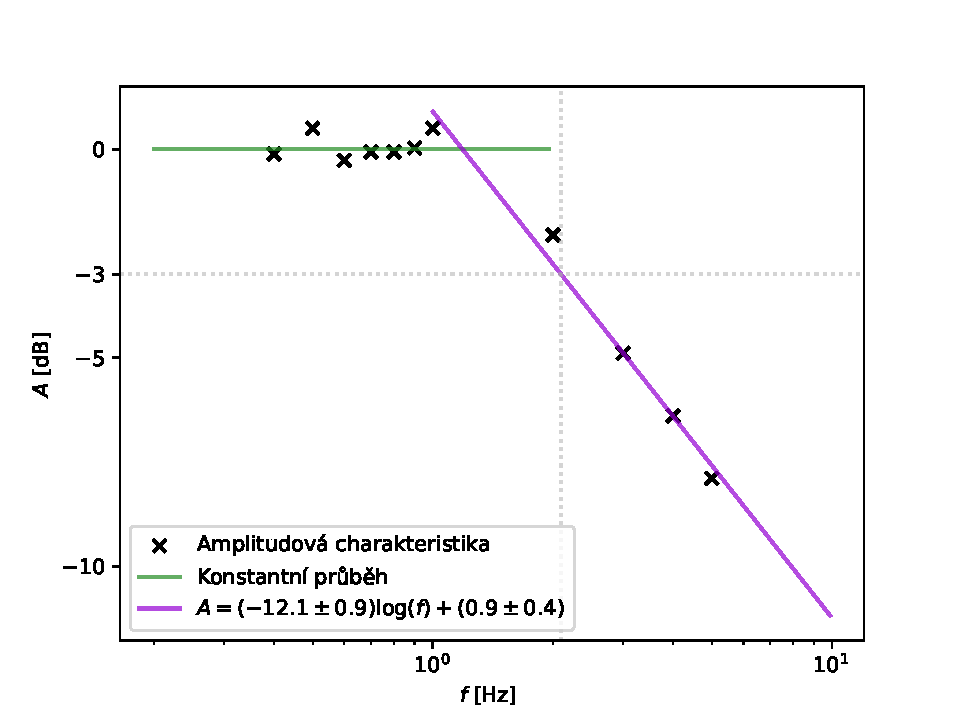
\includegraphics[scale = 0.7]{img/graf_amplitudova_uzavrena.pdf} 
			\caption{Amplitudová frekvenční charakteristika v uzavřené smyčce. Pro frekvence do přibližně 1 Hz je závislost přibližně konstantní, poté se amplituda klesá s funkcí $A=(-12.1\pm 0.9)\log(f)+(0.9\pm 0.4)$.Data byla vycentrována tak, aby konstantní část průbehu byla přibližně na 0 dB.} 
			\label{fig:amplitudova_uzavrena}
		\end{figure}

	\subsection{Metoda \uv{pokus-omyl}}
		Na Obr.~\ref{fig:prechodova_uzavrena_k2} je snímek z osciloskopu zobrazující přechodovou charakteristiku v uzavřené smyčce. Cílem bylo nastavení regulátoru tak, aby  regulační odchylka byla menší než 0.3 a zároveň časová konstanta byla menší než 20 ms. Při nastavení zesílení P regulátoru na $k=2$ byla časová konstanta $T=16\unit{ms}$ a regulační odchylka 0.076 V, což odpovídá zadaným požadavkům.
		
		\begin{figure}[H] 
			\centering
			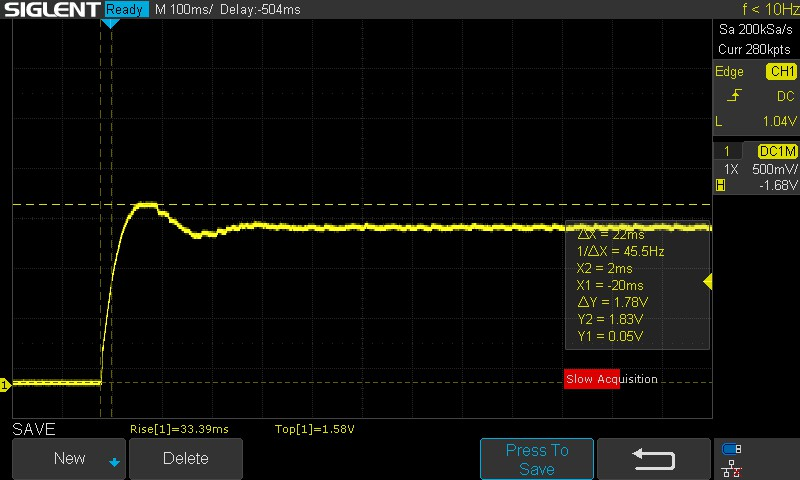
\includegraphics[scale=0.6]{img/SDS00001.jpg} 
			\caption{Snímek z osciloskopu zobrazující přechodovou charakteristiku v uzavřené smyčce. Zesílení P regulátoru bylo $k=2$ byla časová konstanta $T=16\unit{ms}$ a regulační odchylka 0.076 V.} 
			\label{fig:prechodova_uzavrena_k2}
		\end{figure}
		
				
			
% ----------------------------------------------------------------------
%  Diskuse - obsahuje komentář k jednotlivým výsledkům, porovnání s očekáváním/tabulkovými hodnotami, zdroje především systematických chyb měření, návrh na zlepšení výsledků,...
% ----------------------------------------------------------------------			
%	\section{Diskuse}			

% ----------------------------------------------------------------------
%  Závěr - stručně a jasně shrnout splněné cíle měření, úkoly a výsledky měření
% ----------------------------------------------------------------------
			
%\section{Závěr}



